\documentclass{beamer}
\usepackage[UTF8,noindent]{ctexcap}
\usepackage{beamerthemesplit}
\usepackage{diagbox}
\usepackage{graphicx}
\usepackage{float}
\usepackage{amsmath}
\usepackage{geometry}
\usepackage{fontspec}
\usepackage{algorithm}
\usepackage{algorithmicx}
\usepackage{algpseudocode}

\usetheme{Berlin}
\newtheorem{formula}{公式}

\title{基于JESD204B的Serdes接口中接收电路 \\ 设计研究}
\subtitle{论文答辩}
\author{陈登 \\ 导师:姚亚峰}
\date{\today}


\begin{document}

\begin{frame}
	\titlepage
	Power by \LaTeX
\end{frame}

\begin{frame}{目录}
	\tableofcontents
\end{frame}

\section{研究背景}

\begin{frame}{研究背景}{JESD204B接口介绍}
在通信系统中,尤其是无线通信系统,高速AD转换芯片的地位非常重要。伴随着通信系统的传输速率不断飞速增长,传统的AD数据接口,如USB、SPI、I2C,已经远远无法满足在更高速条件下信号传输的需求。

于是一种新的接口技术,JESD204B应运而生,逐渐成为高速AD芯片上的必备接口,在实际中有着广泛的应用。
\end{frame}

\begin{frame}{研究背景}{AD9144}
	\begin{figure}
	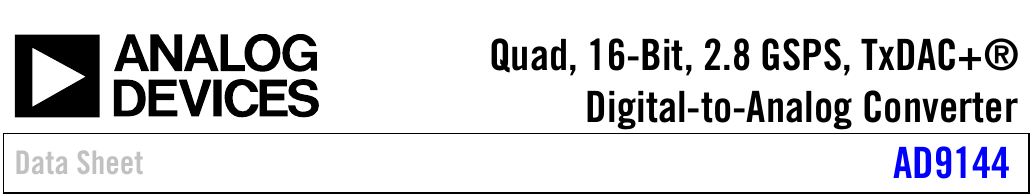
\includegraphics[width=10cm]{./img/ad9144.png}
	\end{figure}
	\begin{block}{}
		$$Max Rate = 4 * 16 * 1.06 = 67.84Gbps$$
		$$Max Lane Rate = Max Rate / 8 = 8.48Gbps$$
	\end{block}
\end{frame}


\begin{frame}{研究背景}{JESD204B协议主要解决的问题}
  \begin{itemize}
    \item 传输高频无线数字信号需要很高的速率。
    \item 所传输的数据需要适用于ADC、DAC的工作方式。
    \item 各大厂商标准化的支持。
  \end{itemize}
\end{frame}

\begin{frame}{研究背景}{JESD204B协议的特点}
  \begin{description}
    \item [新颖] 协议最早制定在2012年,属于硬件接口中的新成员,采用了串行设计。
    \item [高速] 协议规定在子类1条件下能够达到单通道12.5Gbps的传输速率。
    \item [专业] 协议是专门针对ADC、DAC芯片传输需求设计的,充分考虑信号的各种同步、传输情况。
    \item [通用] 协议已经实现在各大芯片公司的高端芯片中,如AD、TI等。
  \end{description}
\end{frame}

\begin{frame}{研究背景}{存在的问题}
现在国内市场上还很少能够看到自主生产的、拥有知识产权的、带有JESD204B接口的ADC、DAC芯片。并且很多现有的芯片并没有采用最新的JESD204B协议。

本课题研究的JESD204B接口接收端电路能够实际应用成为完整JESD204B接口的一部分,具有一定的价值。
\end{frame}

\section{JESD204B协议接收部分}

\begin{frame}{JESD204B协议接收部分}{接收端系统框图}
	\begin{figure}
	\centering
	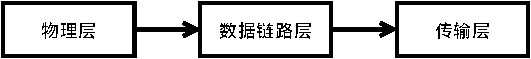
\includegraphics[scale=1]{./img/recv_layer.pdf}
	\caption{接收端系统框图}
	\end{figure}
  \begin{description}
  \item [物理层] SerDes接收端,采用均衡、CDR、CML技术保证高速串行接收。
  \item [链路层] 8B/10B解码器、解扰器、对齐检测。
  \item [传输层] 解帧器。
  \end{description}
\end{frame}

\begin{frame}{JESD204B协议接收部分}{数据链路层}
  8B/10B解码器

  JESD204B协议规定的8B/10B编码主要参考IEEE802.3协议相关部分。
  \begin{itemize}
  \item 编码过程含冗余信息,使传输密度均匀,便于时钟恢复。
  \item 能够保证足够数量的控制字,利于传输过程中帧的构建。
  \item 直流平衡编码,便于有限信道传输,降低功耗,减小误码率。
  \end{itemize}
\end{frame}

\begin{frame}{JESD204B协议接收部分}{数据链路层}
  解扰器
  \begin{figure}
	\centering
	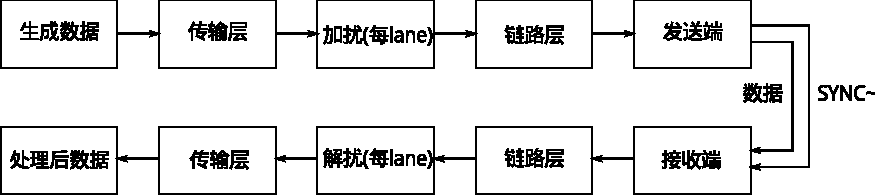
\includegraphics[scale=0.65]{./img/functional_location_of_scrambler_and_descrambler.pdf}
	\caption{解扰器在系统中位置}
	\end{figure}
  \begin{itemize}
  \item 采用自同步扰码,需要一组未加扰数据启动解扰功能。
  \item 增加传输数据随机性,增强数据的信道适应性。
  \end{itemize}
\end{frame}

\begin{frame}{JESD204B协议接收部分}{数据链路层}
  对齐检测
  \begin{itemize}
  \item [CGS] 码群同步,Code Group Synchronization。
  \item [IFS] 初始化帧同步,Initial Frame Synchronization。
  \item [ILS] 初始化lane同步,Initial Lane Alignment Synchronization。
  \end{itemize}
\end{frame}

\begin{frame}{JESD204B协议接收部分}{数据链路层}
  CGS:对链路数据进行检测,判断无效字符数量,在达到错误门限后发起重同步。
  \begin{figure}
	\centering
	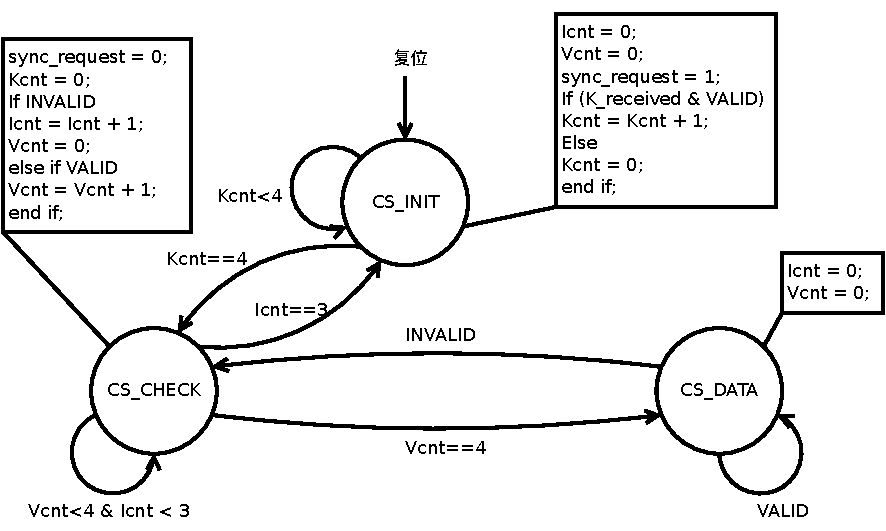
\includegraphics[scale=0.5]{./img/cgs_fsm.pdf}
	\end{figure}
\end{frame}

\begin{frame}{JESD204B协议接收部分}{数据链路层}
  IFS:对链路数据进行检测,关注/F/字符,对齐帧时钟、发起字符替换、检测发端主动重同步。
  \begin{figure}
	\centering
	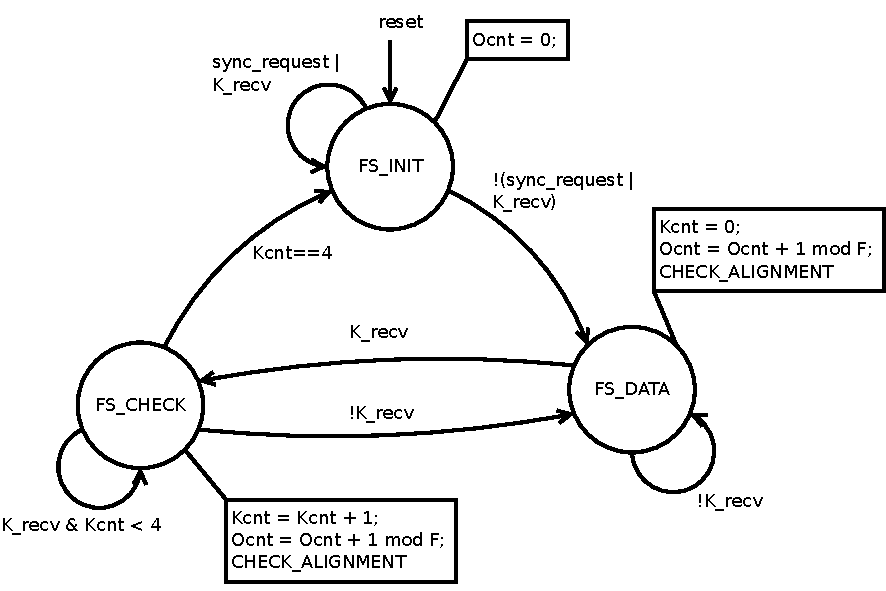
\includegraphics[scale=0.45]{./img/ifs_fsm_resync.pdf}
	\end{figure}
\end{frame}

\begin{frame}{JESD204B协议接收部分}{数据链路层}
  ILS:根据多帧计数判断ILAS位置,给出工作阶段使能信号、替换/A/字符。
  \begin{figure}
	\centering
	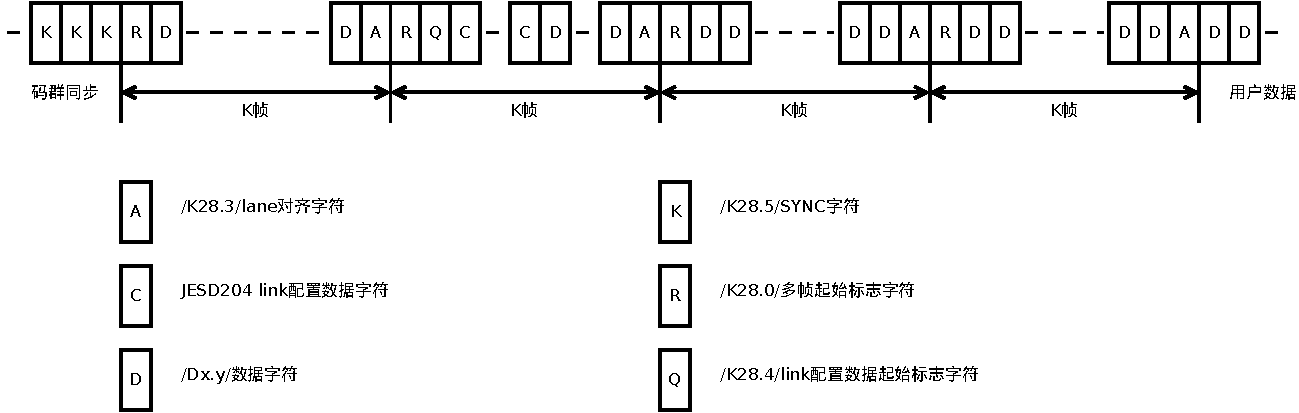
\includegraphics[scale=0.5]{./img/ilas.pdf}
	\end{figure}
\end{frame}

\begin{frame}{JESD204B协议接收部分}{ILAS组成}
  \begin{figure}
  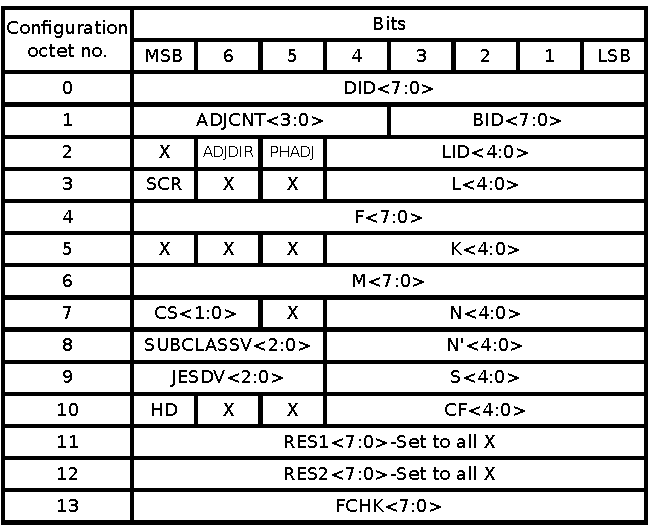
\includegraphics[scale=0.6]{./img/mapping_link_configuration_fields.pdf}
  \end{figure}
\end{frame}

\begin{frame}{JESD204B协议接收部分}{传输层}
  负责将接收到的各个lane数据转换为各个转换器对应的样本数据。
  \begin{figure}
	\centering
	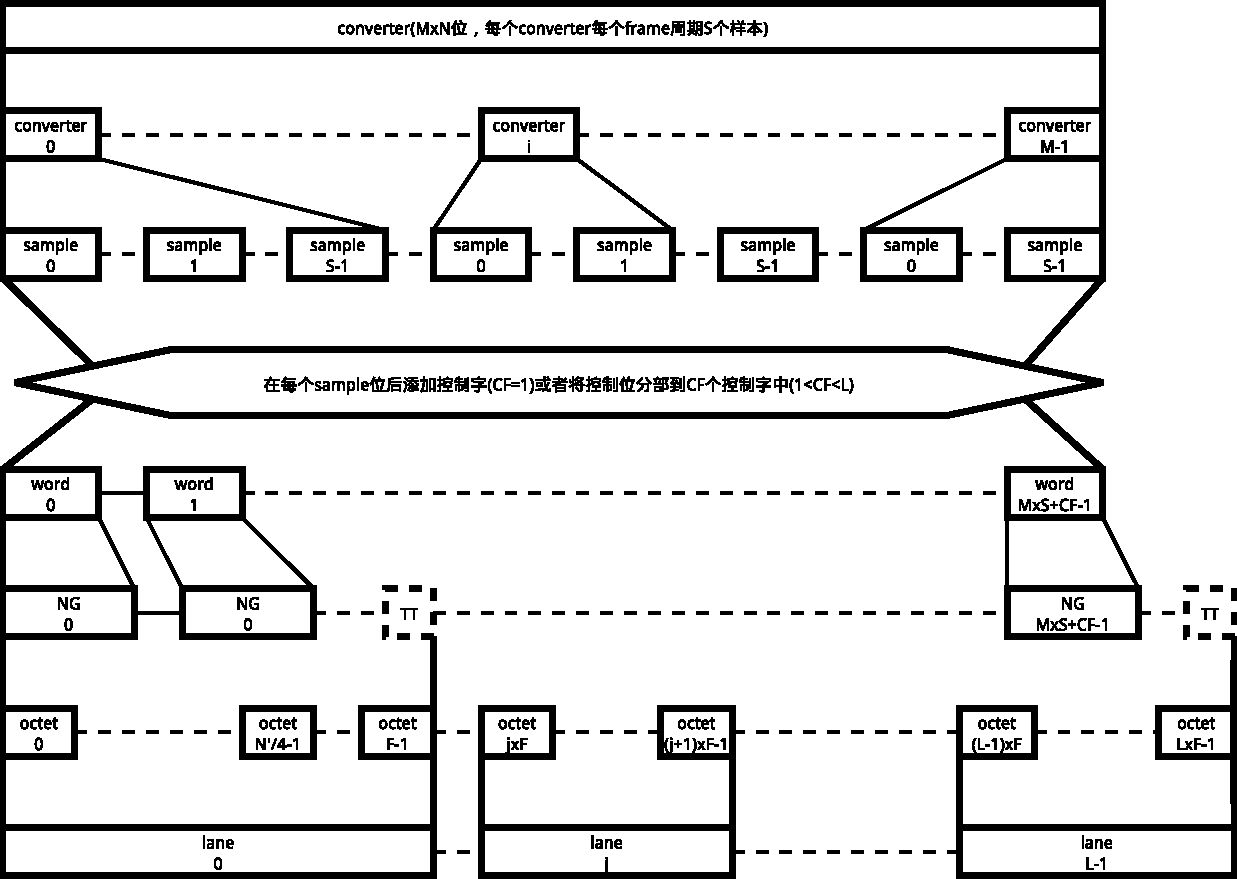
\includegraphics[scale=0.3]{./img/user_data_format_for_multiple_lanes.pdf}
	\end{figure}
\end{frame}

\section{接收部分具体设计}

\begin{frame}{接收部分具体设计}{数据链路层设计框图}
  \begin{figure}
  \centering
  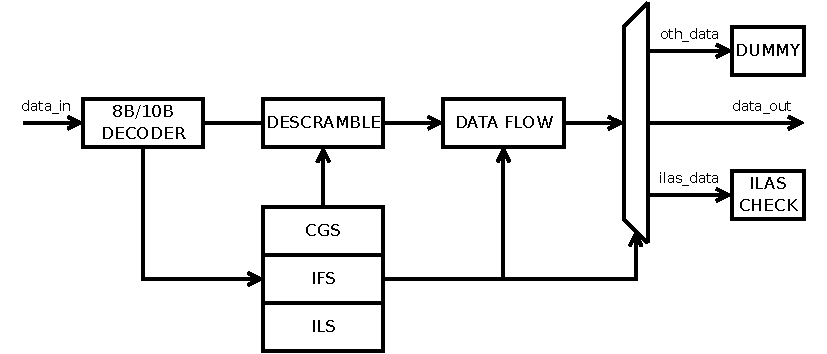
\includegraphics[scale=0.7]{./img/recv_link_layer_top.pdf}
  \caption{接收端数据链路层框图}
  \end{figure}
\end{frame}

\begin{frame}{接收部分具体设计}{8B/10B解码器设计-设计框图}
  \begin{figure}
  \centering
  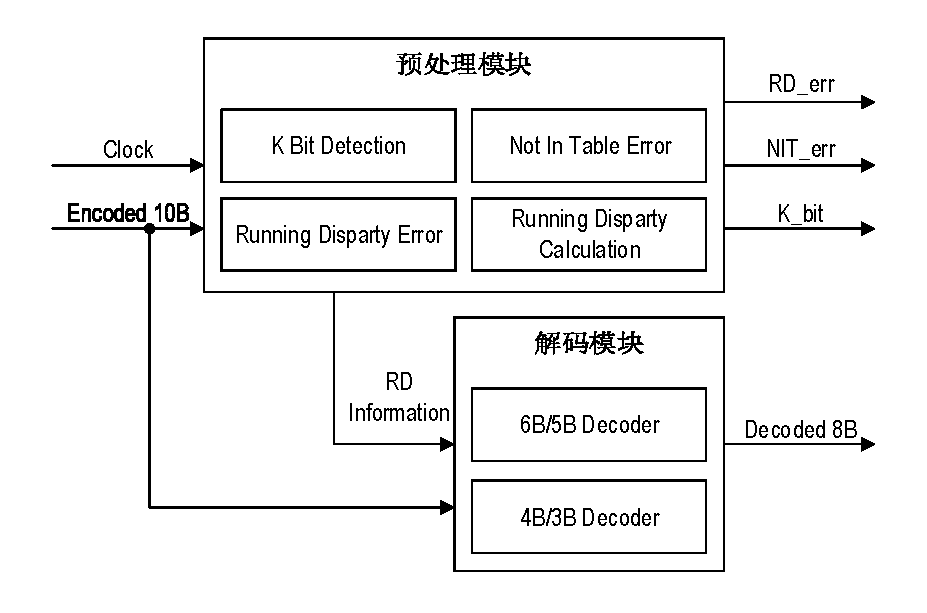
\includegraphics[scale=0.6]{./img/8b10b_decoder_diagram.pdf}
  \end{figure}
\end{frame}

\begin{frame}{接收部分具体设计}{8B/10B解码器设计-预处理部分设计框图}
  \begin{figure}
  \centering
  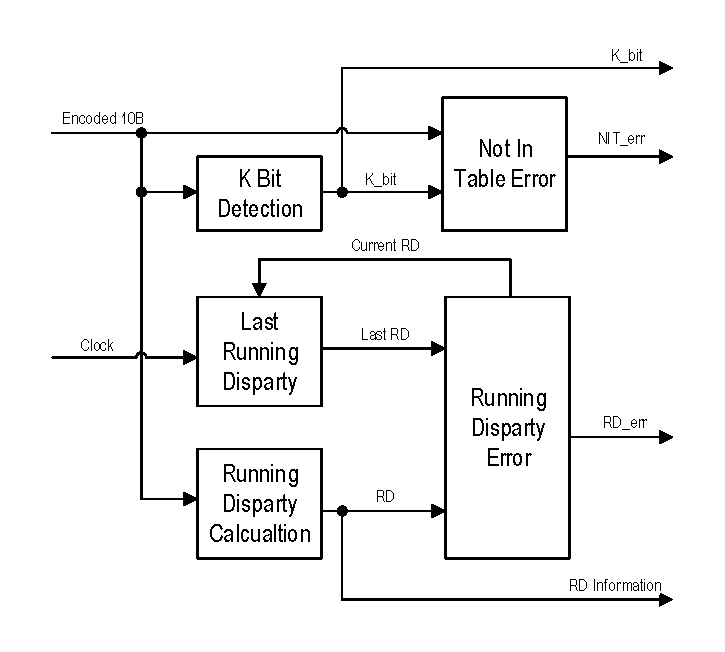
\includegraphics[scale=0.5]{./img/8b10b_preprocess_model.pdf}
  \end{figure}
\end{frame}

\begin{frame}{接收部分具体设计}{8B/10B解码器设计-特色}
	\begin{itemize}
	\item 采用预处理级,直接快速给出极性信息,供解码模块使用,减小解码表设计,减小面积。
	\item 状态机设计的极性跳转设计,提高程序稳定性。
	\item 3B/4B解码与5B/6B解码并列分级进行,充分利用并行特点加快解码速度。
	\end{itemize}
\end{frame}

\begin{frame}{接收部分具体设计}{8B/10B解码器设计-仿真结果}
  \begin{figure}
  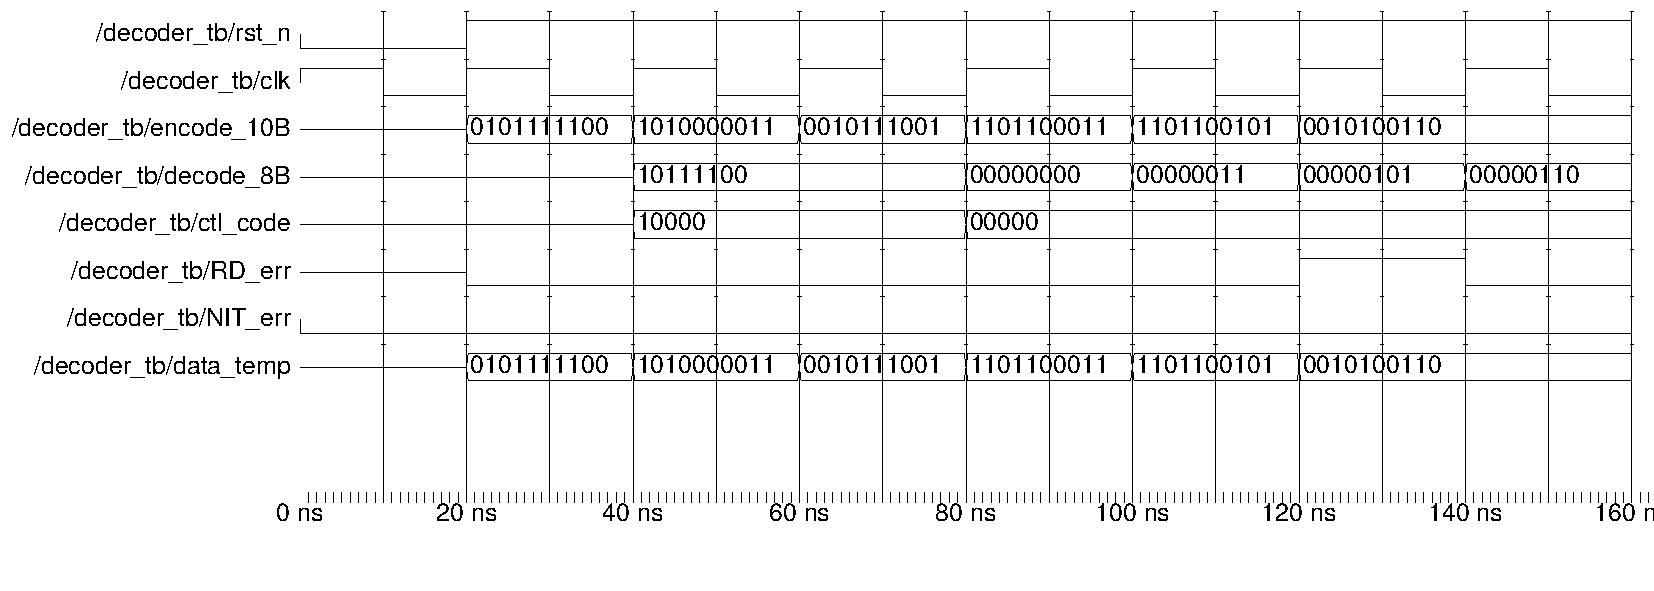
\includegraphics[scale=0.4]{./img/8b_10b_decoder_wave.pdf}
	\caption{8B/10B解码器仿真结果}
  \end{figure}
\end{frame}

\begin{frame}{接收部分具体设计}{8B/10B解码器设计-综合结果}
  \begin{table}[H]
  \centering
  \begin{tabular}{|c|r|r|r|}
  \hline
  \diagbox{项目}{设计}       & Classic     & Actel        & New   \\
  \hline
  Total Cell Area($\mu m^2$) & 1716(98\%)	 & 2657(151\%)  &	1759	\\
  \hline
  Timing($ns$)					     & 8.16        & 9.97         & 9.54 	\\
  Time Used($ns$)				     & 5.84        & 4.03         & 4.46	\\
  \hline
  Frequency($MHz$)           & 171.2(76\%) & 248.1(111\%) &	224.2 \\
  \hline
  Total Dynamic Power($nW$)	 &	65.4(81\%) & 81.1(101\%)  & 80.5  \\
  \hline
  \end{tabular}
  \end{table}
\end{frame}

\begin{frame}{接收部分具体设计}{解扰器设计-解扰公式}
	\begin{equation}
		\begin{cases}
			D_{31} = S_{31} + S_{17} + S_{16} \\
			D_{30} = S_{30} + S_{16} + S_{15} \\
			\dots							  \\
			D_{17} = S_{17} + S_{3} + S_{2}   \\
			D_{16} = S_{16} + S_{2} + S_{1}   \\
		\end{cases}
	\end{equation}
\end{frame}

\begin{frame}{接收部分具体设计}{解扰器设计-解扰器并行实现}
  \begin{figure}
  \centering
  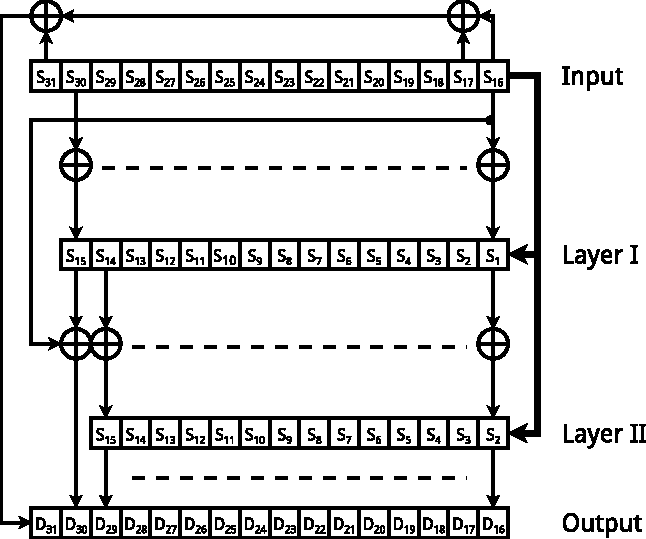
\includegraphics[scale=0.5]{./img/scrambler_descrambler_parallel_implementation.pdf}
  \end{figure}
\end{frame}

\begin{frame}{接收部分具体设计}{解扰器设计-特色}
	\begin{itemize}
	\item 采用两级缓冲处理,通过流水的设置以面积换解扰速率。
	\item 能够以32比特进行并行处理,降低处理频率。
	\item 自同步要求先存有未加扰数据作为种子,第一级处理保留了未加扰数据。
	\end{itemize}
\end{frame}

\begin{frame}{接收部分具体设计}{对齐检测设计-CGS流程}
  \begin{figure}
  \centering
  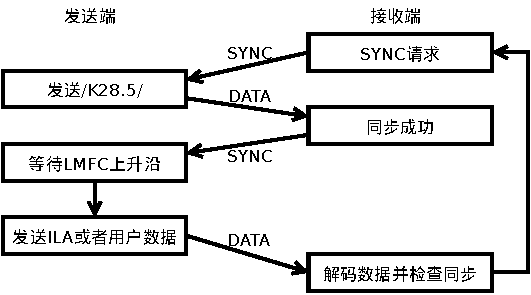
\includegraphics[scale=0.8]{./img/cgs_subclass_1_2.pdf}
  \end{figure}
\end{frame}

\begin{frame}{接收部分具体设计}{对齐检测设计-CGS流程}
  \begin{enumerate}
  \item 当链接启动,接收端发送同步请求,发送端传回/K28.5/。
  \item 正确接收另外4个/K28.5/字符后接收端认为码群同步完成。
  \item 当收到错误码字后,接收端进入“CHECK”状态。
  \item 如果又有3个错误码字在“CHECK”状态被接受,就表示失去同步。
  \item 如果在“CHECK”状态连续收到4个正常码字,则进入正常状态。
  \end{enumerate}
\end{frame}

\begin{frame}{接收部分具体设计}{对齐检测设计-CGS仿真结果}
  \begin{figure}
  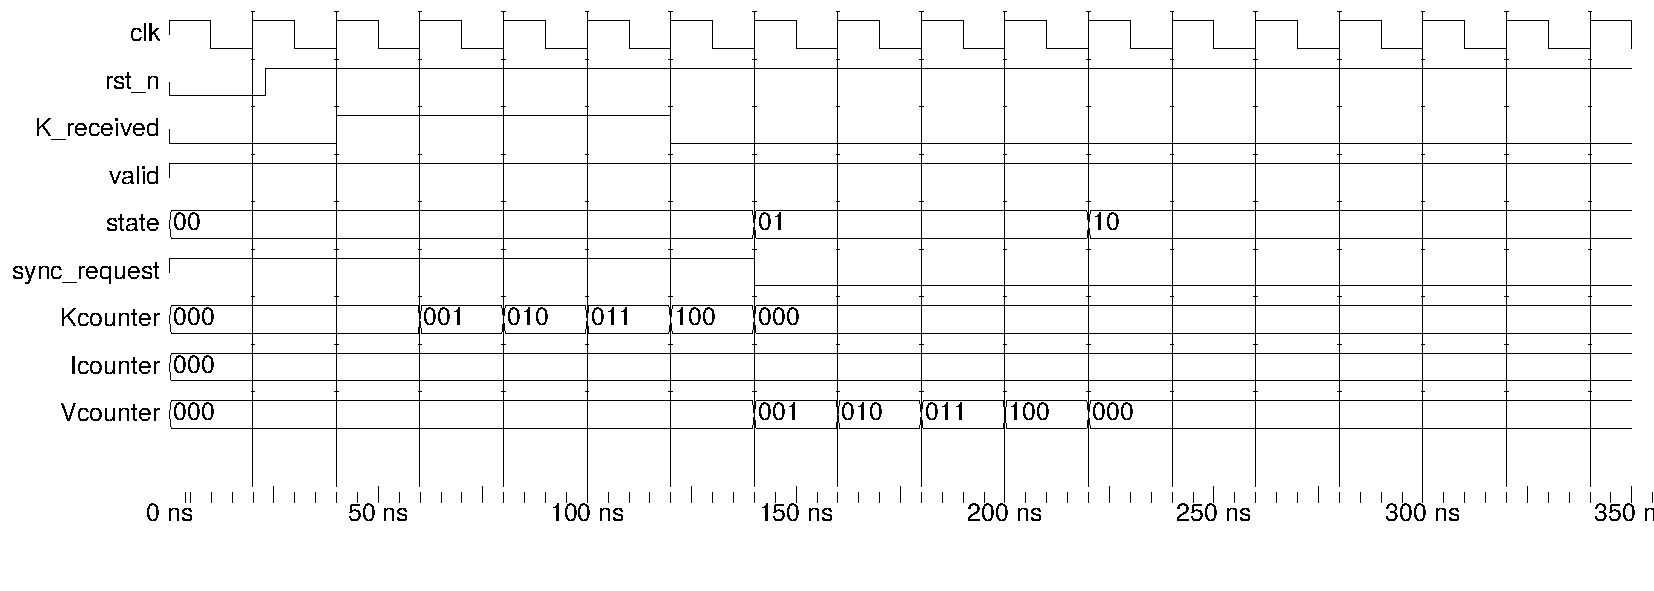
\includegraphics[scale=0.4]{./img/cgs_detection_wave.pdf}
  \end{figure}
\end{frame}

\begin{frame}{接收部分具体设计}{对齐检测设计-IFS流程}
  当一个link启动时,帧同步的由以下几点实现:
  \begin{itemize}
    \item 在码群同步过程中,发送端会一直发送/K28.5/的逗点符号。
    \item 在码群同步结束后,收端会假设收到第一个非/K28.5/符号作为帧的开始。如果发送端开始发送ILAS,那么第一个非/K28.5/字符就是/K28.0/字符。
    \item 接收端假设在每F个octet后就是新的一帧的开始。
  \end{itemize}
\end{frame}

\begin{frame}{接收部分具体设计}{对齐检测设计-帧对齐和帧纠错}
  \begin{algorithmic}
  	\If{(A\_recv | F\_recv)}
  		\State REPLACE\_ALIGNMENT\_CHARACTER;
  		\If{((Ocnt == previous\_AF\_position) \& VALID)}
  			\State RESET\_OCTET\_COUNTER;
  		\EndIf
  		\If{VALID | (Ocnt == F-1)}
  			\State previous\_AF\_position = Ocnt;
  		\EndIf
  	\EndIf
  \end{algorithmic}
\end{frame}

\begin{frame}{接收部分具体设计}{对齐检测设计-ILS流程}
  当一个link启动时,lane同步的由以下几点实现:
  \begin{itemize}
    \item 对ILAS序列的检测、分析工作和lane的监测工作。
    \item 完成了初始化帧同步后紧接着的就是初始化lane对齐的工作。
    \item 初始化lane对齐完成后就需要对lane进行监控,判断是否需要重对齐。
  \end{itemize}
\end{frame}

\begin{frame}{接收部分具体设计}{对齐检测设计-lane对齐和lane纠错}
  \begin{algorithmic}
  	\If{A\_recv}
  		\State REPLACE\_A;
  		\If{((Fcnt == previous\_A\_position) \& VALID)}
  			\State RESET\_FRAME\_COUNTER;
  		\EndIf
  		\If{VALID | (Fcnt == F-1)}
  			\State previous\_A\_position = Fcnt;
  		\EndIf
  	\EndIf
  \end{algorithmic}
\end{frame}



\begin{frame}{接收部分具体设计}{对齐检测设计-IFS/ILS仿真结果}
  \begin{figure}
  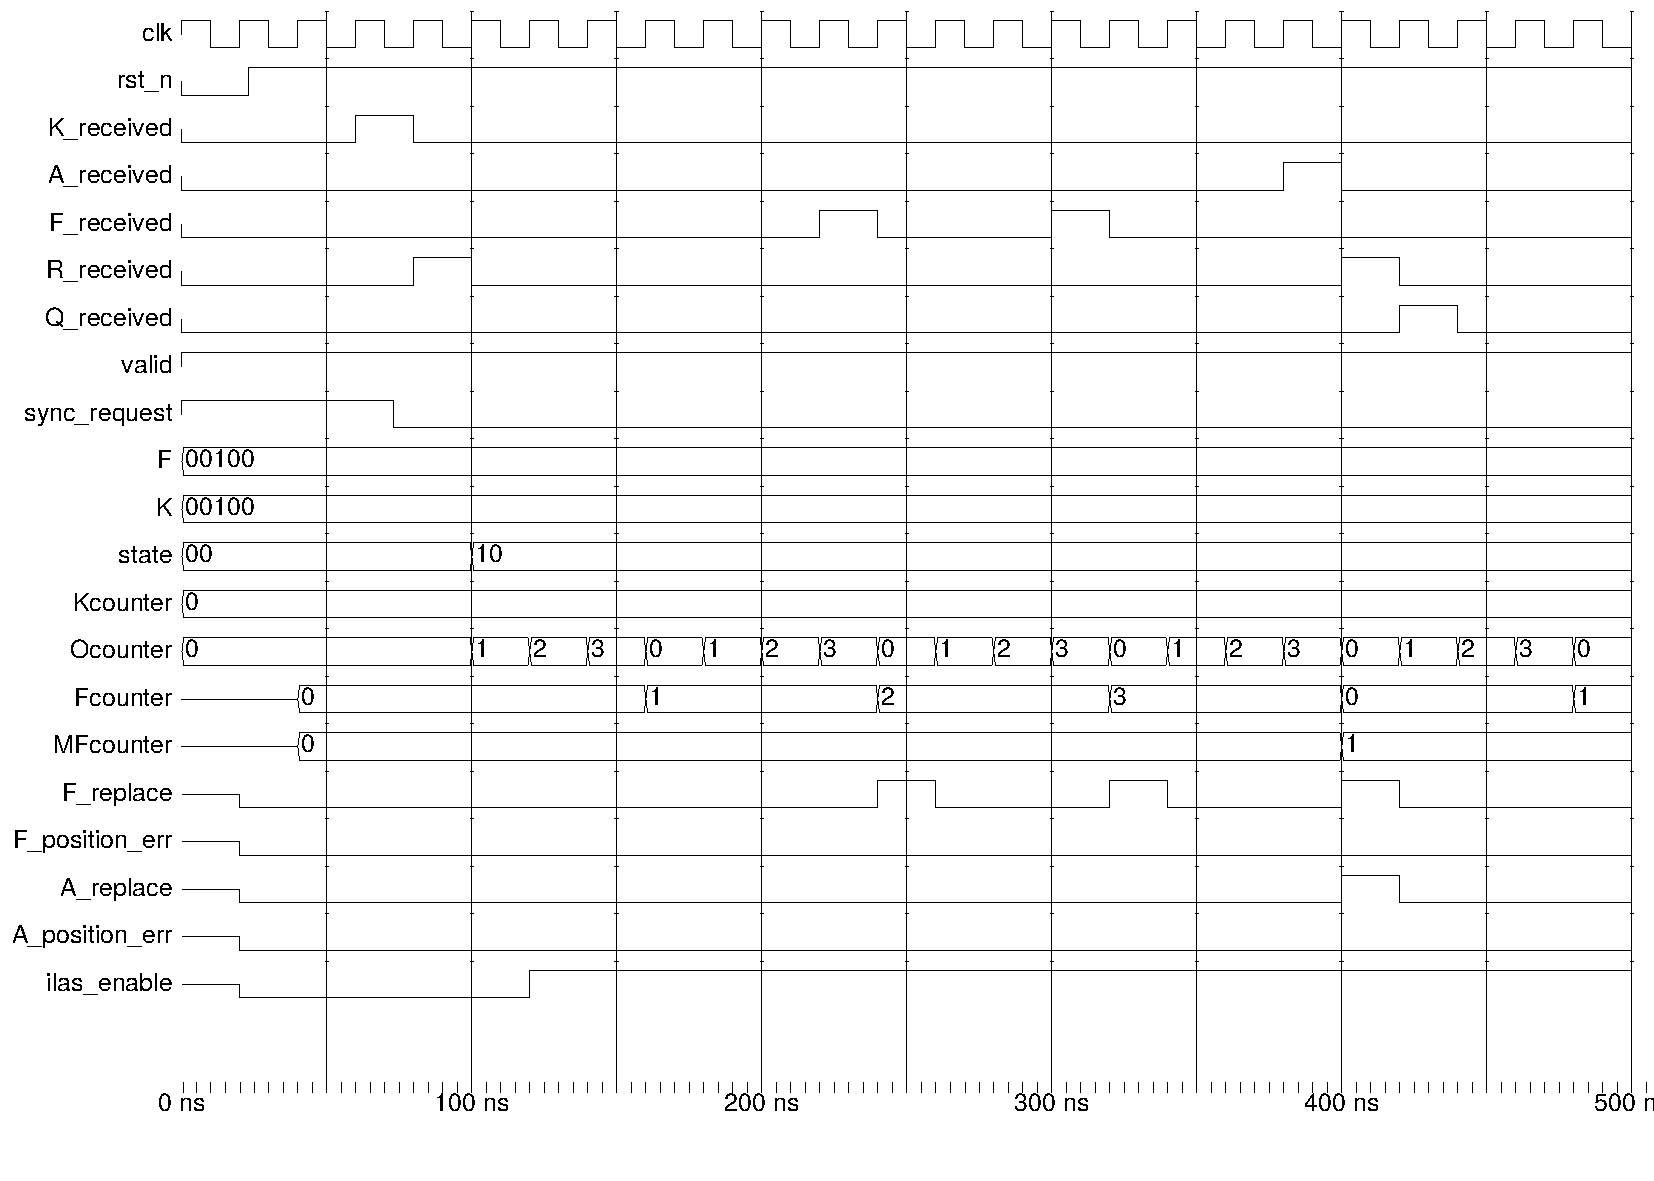
\includegraphics[scale=0.3]{./img/ifs_detection_wave.pdf}
  \end{figure}
\end{frame}

\begin{frame}{接收部分具体设计}{对齐检测设计-数据流仿真结果}
  \begin{figure}
  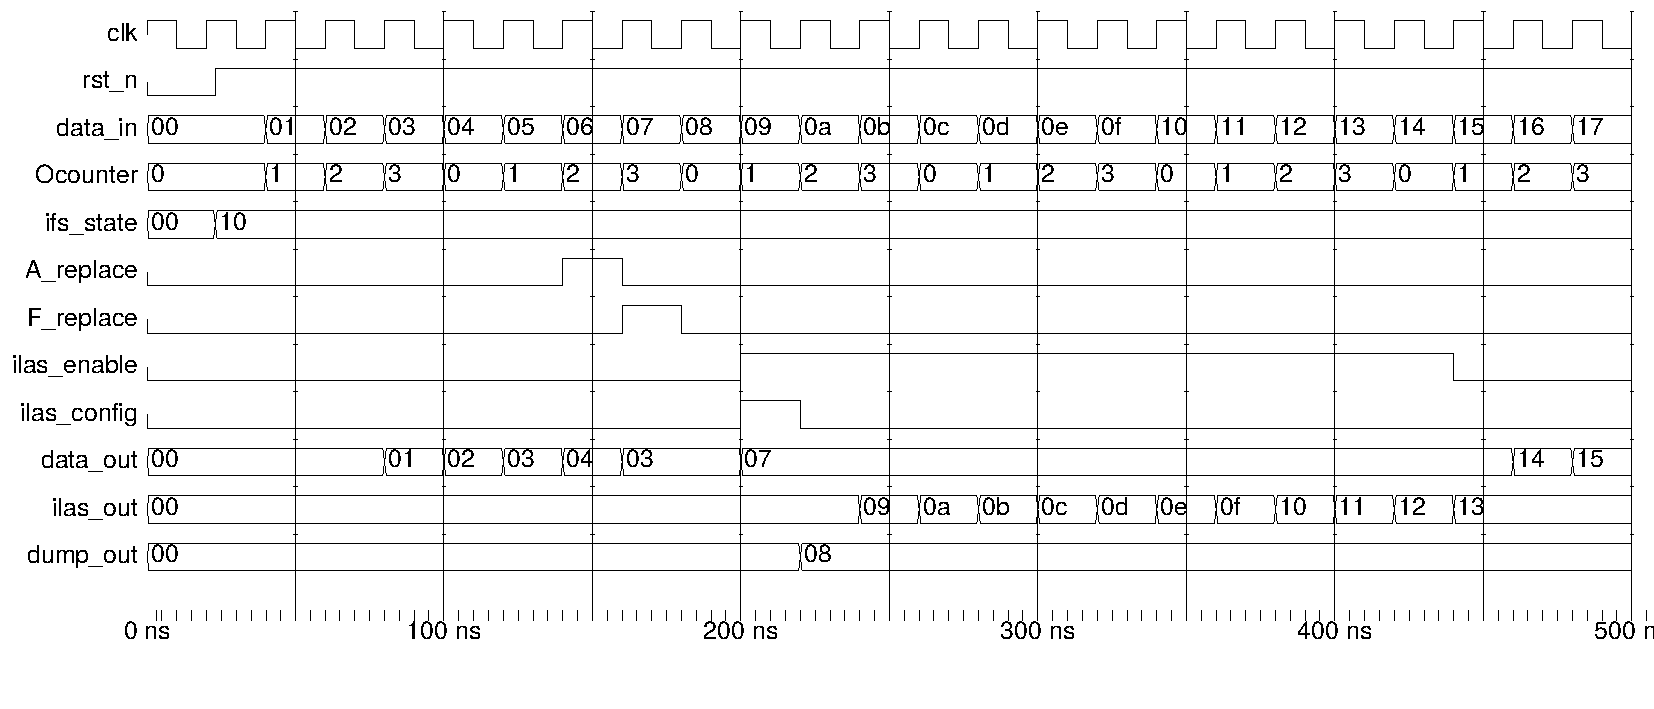
\includegraphics[scale=0.4]{./img/data_flow_wave.pdf}
  \end{figure}
\end{frame}

\begin{frame}{接收部分具体设计}{对齐检测设计-综合结果}
  \begin{table}[H]
  \centering
  \begin{tabular}{|c|r|r|r|}
  \hline
  \diagbox{项目}{设计} & ILS/IFS & DATA FLOW \\
  \hline
  Total cell Area($\mu m^2$) & 8718 & 4966 \\
  \hline
  Timing($ns$)					   & 3.71 & 7.96 \\
  Time Used($ns$)					 & 6.15 & 1.99 \\
  \hline
  Frequency($MHz$)				&	162.6 & 502.5 \\
  \hline
  Total Dynamic Power($nW$)		&	535.6	& 490.9 \\
  \hline
  \end{tabular}
  \end{table}
\end{frame}

\begin{frame}{接收部分具体设计}{对齐检测设计-级联仿真结果}
  \begin{figure}
  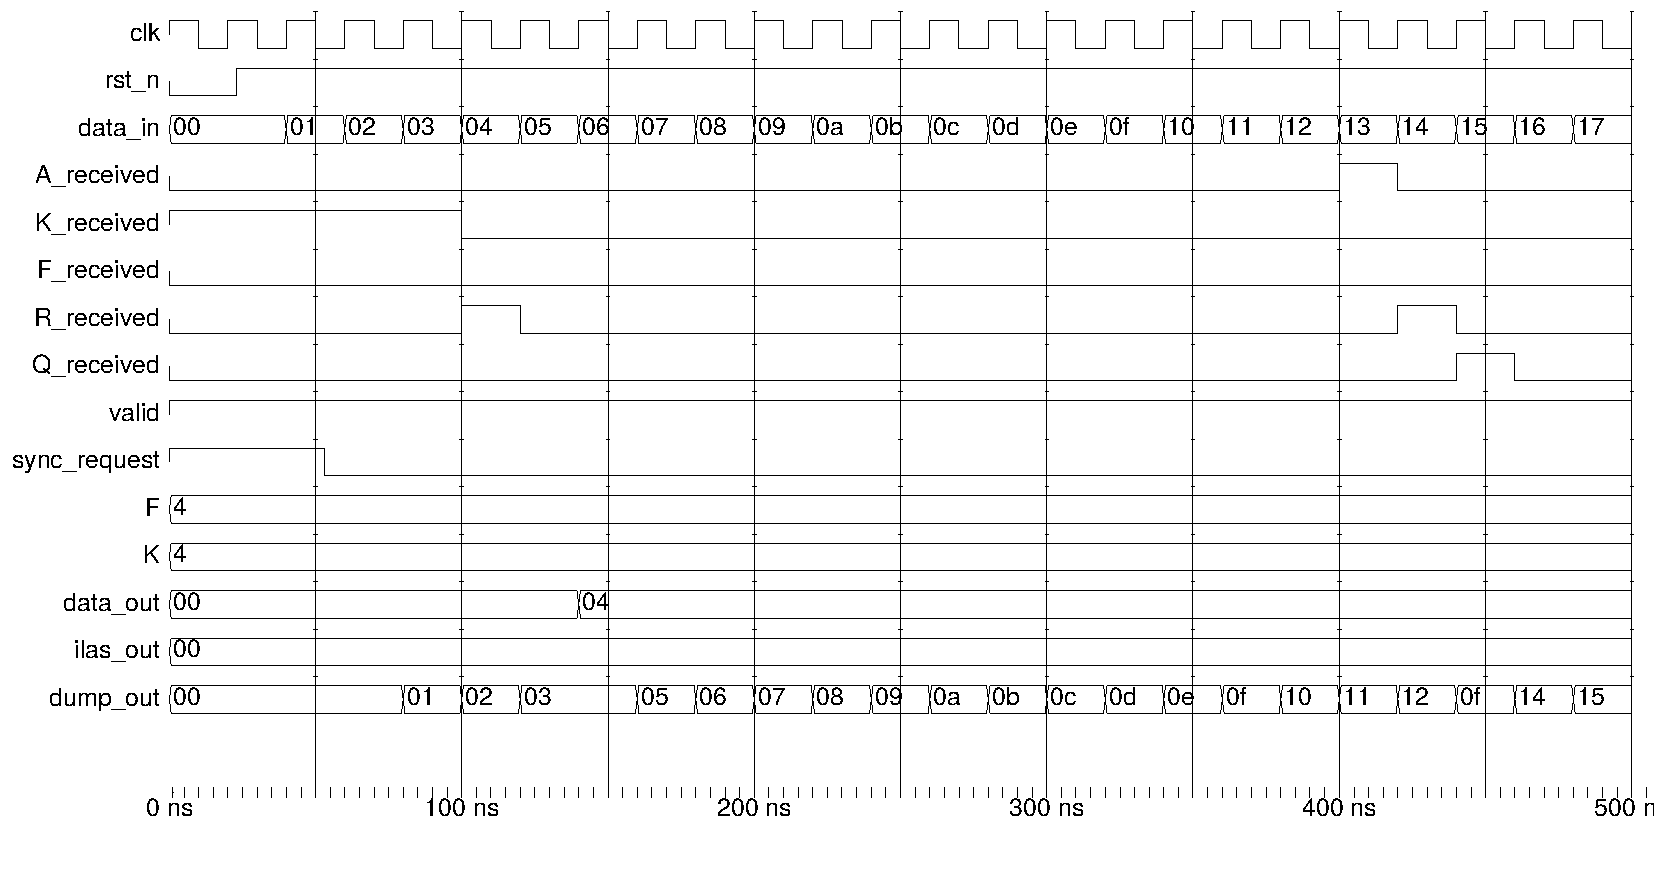
\includegraphics[scale=0.35]{./img/recv_top_wave.pdf}
  \end{figure}
\end{frame}

\section{总结}

\begin{frame}{总结}{设计结果}
	本文的主要完成的工作是设计通信接口的接收端电路,包括
	\begin{itemize}
	\item 8B/10B解码器设计
	\item 解扰器设计
	\item 码群同步状态机设计
	\item 初始化lane同步状态机设计
	\item 初始化帧同步状态机设计
  \item 数据流模块设计
	\end{itemize}
\end{frame}

\begin{frame}{总结}{芯片设计流程}
	\begin{enumerate}
	\item 分析协议接收端相关设计要求,结合已有相关芯片数据手册,得到合理的设计思路。
  \item 采用Verilog语言RTL级设计。
	\item Verdi3错误检查。
	\item Modelsim仿真。
	\item Design Compiler配合SMIC 180nm工艺库进行综合,得到逻辑仿真结果和电路综合结果。
  \end{enumerate}
\end{frame}

\begin{frame}{总结}{芯片设计结果}
	\begin{itemize}
	\item 实现的码群同步状态机单元面积为1500$\mu m^2$,工作频率可达1GHz。
	\item 初始化lane同步状态机单元面积为8700$\mu m^2$,工作频率可达162MHz。
	\item 数据流模块单元面积为5000$\mu m^2$,工作频率可达500MHz。
	\item 8B/10B解码器模块单元面积为1759$\mu m^2$,工作频率可达224MHz。
	\end{itemize}
\end{frame}

\begin{frame}{谢谢}{}
	\centering
	请各位专家、教授提问!谢谢!
\end{frame}

\end{document}
